\icode{O-EX-SU261001}
游标卡尺构造：无论哪种分度的游标卡尺，游标尺都比主尺短\qty{1}{mm}。
	\begin{table}[h]
		\centering
		\begin{tblr}{|c|c|c|c|}
		\hline
		副尺规格&总长&每格长度&精确度\\
		\hline
		10格副尺&\qty{9}{mm}&\qty{0.9}{mm}&\qty{0.1}{mm}\\
		\hline
		20格副尺&\qty{19}{mm}&\qty{0.95}{mm}&\qty{0.05}{mm}\\
		\hline
		50格副尺&\qty{49}{mm}&\qty{0.98}{mm}&\qty{0.02}{mm}\\
		\hline
		\end{tblr}
	\end{table}

	\begin{figure}[htbp]
		\centering
		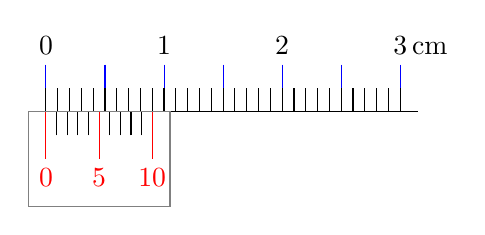
\begin{tikzpicture}[scale=1.5]
			\draw (-.6,0)--(2.7,0);
			\foreach \x in {-.45,0.05,...,2.55}
				\draw[blue] (\x,.4)--(\x,0);
			\foreach \x/\n in {-.45/0,0.55/1,1.55/2,2.55/3}
				\node at(\x,.4)[above]{\(\n\)};
			\foreach \x in {-.45,-.35,...,2.55}
				\draw (\x,.2)--(\x,0);
			\draw[gray] (-.6,-.8) rectangle(.6,0);
			\foreach \x in {-.45,-.36,...,.45}
				\draw (\x,-.2)--(\x,0);
			\foreach \x/\n in {-.45/0,0/5,.45/10}
				\draw[red] (\x,-.4)node[below]{\(\n\)}--(\x,0);
			\node at(2.8,.4)[above]{\qty{}{cm}};
		\end{tikzpicture}
	\end{figure}

	\begin{figure}[htbp]
		\centering
		\begin{tikzpicture}[scale=1.5]
			\foreach \x in{-2.7,0}
				\draw[dashed] (\x,1)--(\x,-1);
			\draw[dashed] (-.45,0)--(-.45,-1);
			\draw[|<->|] (-2.7,.9)--node[fill=white]{\footnotesize 主尺准确值}(0,.9);
			\draw[|<->|] (-2.7,-.3)--node[fill=white]{\footnotesize 待测物实际长度}(-.45,-.3);
			\draw[|<->|] (-.45,-.9)--node[below]{\footnotesize 游标尺长度}(0,-.9);
			\draw (-2.8,0)--(.8,0);
			\foreach \x/\n in {.3/3,-.7/2,-1.7/1,-2.7/0}
				\node at(\x,.4)[above]{\(\n\)};
			\foreach \x in {.3,-.2,...,-2.7}
				\draw[blue] (\x,.4)--(\x,0);
			\foreach \x in {.7,.6,...,-2.7}
				\draw (\x,.2)--(\x,0);
			
			\foreach \x in {-.45,-.36,...,.45}
				\draw (\x,-.2)--(\x,0);
			\foreach \x/\n in {-.45/0,0/5,.45/10}
				\draw[red] (\x,-.4)node[below]{\(\n\)}--(\x,0);
			\node at(.6,.4)[above]{\qty{}{cm}};
		\end{tikzpicture}
	\end{figure}